\documentclass{beamer}

\usepackage{amsmath, amssymb}
\usepackage{tikz-cd}
\usepackage{xcolor}
\usepackage{graphicx}

\title{MAT102 - College Algebra - Polynomial and Rational Functions}
\subtitle{3.1 Quadratic Functions and Applications \cite{miller2016college}}
\author{\textbf{Miraj Samarakkody}}
\institute{Tougaloo College}
\date{Updated - \today}

\begin{document}

\begin{frame}
    \titlepage
\end{frame}

\begin{frame}{Graph a Quadratic Function Written in Vertex Form}
    \begin{itemize}
        \item A function of the form \(f(x) =mx+c ~ (m \ne 0)\) is a linear function. \pause
        \item The function defined by \(f(x) = ax^2 +bx + c ~(a \ne 0) \) is called a \textbf{quadratic function.}  \pause
    \end{itemize}
    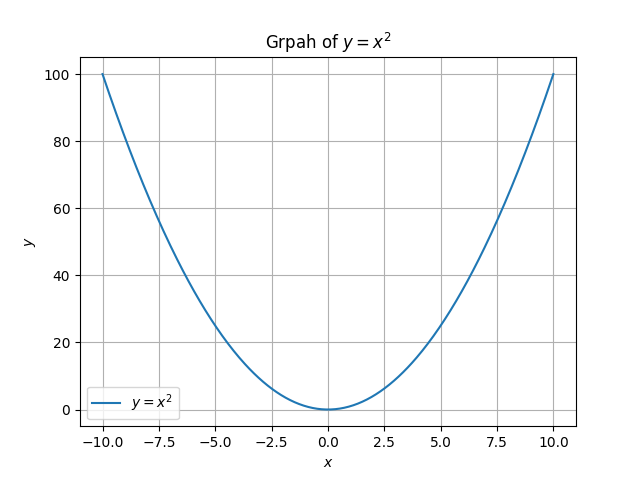
\includegraphics[scale=0.5]{figs/Figure_1.png}\pause
\end{frame}

\begin{frame}
    \frametitle{Graph a Quadratic Function Written is Vertex Form}
    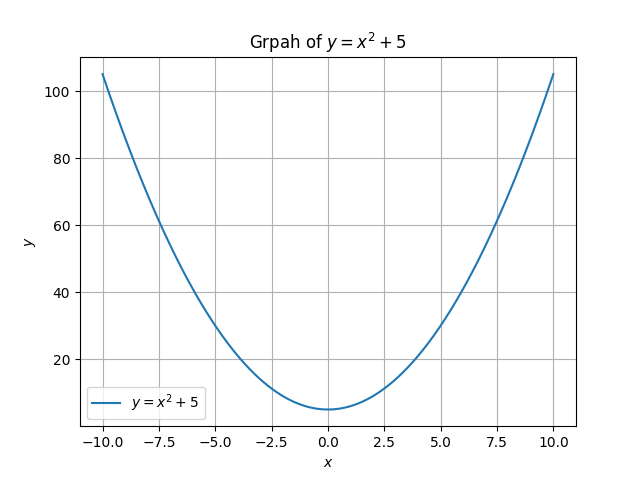
\includegraphics[scale=0.5]{figs/Figure_2.png}

    

\end{frame}

\begin{frame}
    \frametitle{Graph a Quadratic Function Written is Vertex Form}
    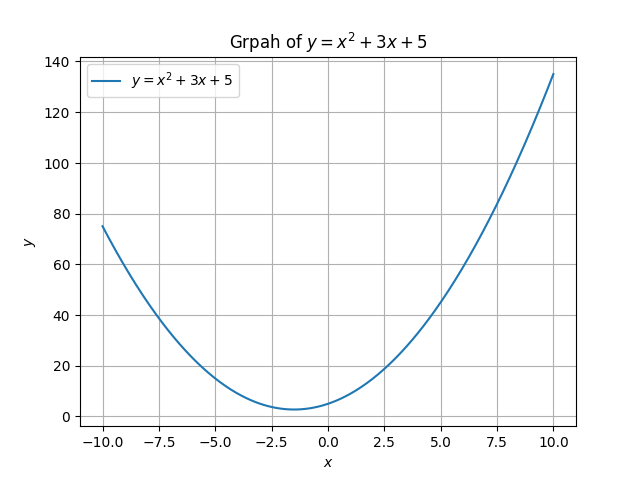
\includegraphics[scale=0.5]{figs/Figure_3.png}
\end{frame}

\begin{frame}
    \frametitle{Quadratic Function}

    A function defined by \(f(x) = ax^2 +bx +c~ (a \ne 0)\) is called a \textbf{quadratic function}. By completing the square, \(f(x)\) can be expressed in \textbf{vertex form} as \(f(x)= a(x-h)^2+k\).\pause
    \begin{itemize}
        \item The graph of \(f\) is a parabola with vertex \((h,k)\). \pause
        \item If \(a>0\), the parabola opens upward, and the vertex is the minimum point. The minimum value of \(f\) is \(k\). \pause
        \item If \(a<0\), the parabola opens downward, and the vertex is the maximum point. The maximum value of \(f\) is \(k\). \pause
        \item The axis of symmetry is \(x=h\). This is the vertical line that passes through the vertex. 
    \end{itemize}

\end{frame}

\begin{frame}{Example - Analyzing and Graphing a Quadratic Function}
Given \(f(x)=-2(x-1)^2+8\),
\begin{enumerate}
    \item Determine whether the graph of the parabola opens upward or downward. \pause
    \item Identify the vertex. \pause 
    \item Determine the \(x-\)intercepts. \pause 
    \item Determin the \(y-\)intercepts. \pause
    \item Sketch the function. \pause
    \item Determine the axis of symmetry. \pause  
    \item Determine the maximum or minimum value of \(f\).\pause
    \item Write down the domain and range in interval notaion. 
\end{enumerate} 

    
\end{frame}

\begin{frame}
    \frametitle{Example - Writing a Quadratic Function in Vertex Form}

    Given \(f(x)=3x^2 +12x+5\),

    \begin{enumerate}
        \item Write the function in vertex form. \pause
        \item Identify the vertex. \pause
        \item Identify the \(x-\)intercept.\pause
        \item Identify the \(y-\)intercept. \pause
        \item Sketch the function.\pause
        \item Determine the axis of symmetry. \pause
        \item Determine the minimum or maximum value of \(f\). \pause
        \item Write the domain and range in interval notation. 
    \end{enumerate}

\end{frame}

\begin{frame}
    \frametitle{Vertex Formula to Find the Vertex of a Parabola}

    For \(f(x)=ax^2 +bx +c ~(a \ne 0 )\), the vertex is given by \[\left(\dfrac{-b}{2a},f \left(\dfrac{-b}{2a}\right)\right)\]

    

\end{frame}
\begin{frame}
    \frametitle{Example - Using the Vertex Formula}

    Given \(f =-x^2 +4x -5\),
    \begin{enumerate}
        \item State whether the graph of the parabola opens upward or downward. \pause
        \item Determine the vertex of the parabola by using the vertex formula. \pause
        \item Determine the \(x-\)intercepts. \pause
        \item Determine the \(y-\)intercepts. \pause
        \item Sketh the graph. \pause
        \item Determine the axis of symmetry.  \pause
        \item Determine the minimmum or maximum value of \(f\). \pause
        \item Write the domain and range in interval notation. 
    \end{enumerate} 

\end{frame}

\begin{frame}
    \frametitle{Using the Discriminant to Determine the Number of \(x-\)Intercepts}

    Given a quadratic function defined by \(f(x)= ax^2 +bx +c ~(a \ne 0)\), \pause
    \begin{itemize}
        \item If \(b^2 -4ac =0\), the graph of \(y=f(x)\) has one \(x-\)intercept. \pause
        \item If \(b^2 -4ac >0\), the graph of \(y=f(x)\) has two \(x-\)intercept. \pause
        \item If \(b^2 -4ac < 0\), the graph of \(y=f(x)\) has no \(x-\)intercept. 
    \end{itemize}

\end{frame}

\begin{frame}
    \frametitle{Example - Using a Quadratic Function for Projectile Motion}

    A stone is thrown from a 100-m cliff at an initial speed of \(20\) m/sec at an angle of \(30^0\) from the horizontal. The height of the stone can be modeled by \(h(t)=-4.9t^2 +10t +100\), where \(h(t)\) is the height in meters and \(t\) is the time in seconds after the stone is released. 
    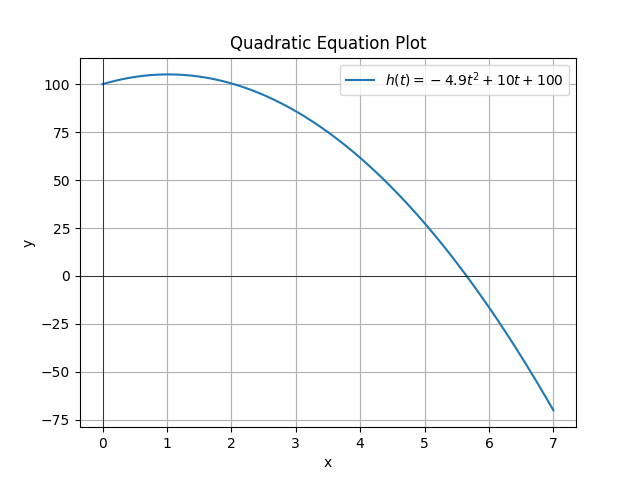
\includegraphics[scale=0.2]{figs/Figure 4.png} 

    \begin{enumerate}
        \item Determine the time at which the stone will be at its maximum height.\pause
        \item Determine the maximum height. \pause
        \item Determine the time at which the stone will hit the ground. 
    \end{enumerate}

\end{frame}

\begin{frame}
    \frametitle{Example - Applying a Quadratic Function to Geometry}

    A parking area is to be constructed adjacent to a road. The develper has purchased 340 ft of fencing. Determine dimesions for the parking lot that would maximize the area. Then find the maximum area. \\
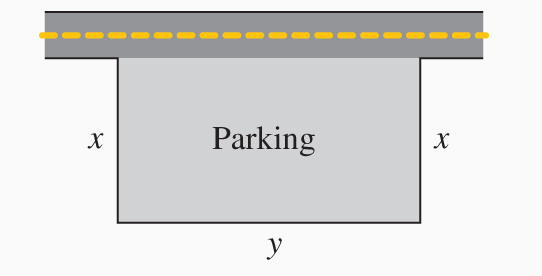
\includegraphics[scale=0.5]{figs/Figure 5.PNG}

\end{frame}

\begin{frame}
    
\end{frame}



\begin{frame}
    \frametitle{References}
    \bibliographystyle{plain} % or another style like unsrt, alpha, etc.
    \bibliography{reference}  % omit the .bib extension
\end{frame}

\end{document}

